\documentclass[12pt,a4paper]{article}
\usepackage[utf8]{vietnam}
\usepackage{amsmath,amssymb}
\usepackage{tabularx}
\usepackage{tikz}
\usepackage{xcolor}
\usepackage[top=0.6cm, bottom=0.6cm, left=0.6cm, right=0.6cm]{geometry}
\usepackage[dethi]{ex_test}

\SAOPTN{widthSA=2.6,heightSA=0.62}
\setlength{\parskip}{0pt}

% Dong ke cham mo chuan viet tay
\newcommand{\dongke}[1]{%
  \begingroup%
  \setlength{\parskip}{0pt}%
  \baselineskip=18.5pt%
  \vspace{1.0mm}%
  \foreach \i in {1,...,#1}{%
    \noindent{\color{gray!60}\dotfill}\par%
  }%
  \vspace{0.6mm}%
  \endgroup%
}

% Khu vuc bai lam chia 2 cot co vach ngan mo o giua
\newcommand{\dongkeHaiCot}[1]{%
  \par\vspace{0.5mm}%
  \noindent%
  \begin{minipage}[t]{0.485\linewidth}%
    \dongke{#1}%
  \end{minipage}%
  \hfill%
  {\color{gray!60}\vrule}%
  \hfill%
  \begin{minipage}[t]{0.485\linewidth}%
    \dongke{#1}%
  \end{minipage}%
}

% Dinh nghia o bai tap tu luan trong bang
\newcommand{\oBaiTap}[3][5]{%
  \vspace{1.0mm}%
  \noindent\textbf{#2} #3\par%
  \dongke{#1}%
}

\begin{document}
\pagestyle{empty}
% =============================================================================
% ========================= TOAN 8 TUAN 09 BUOI 01 - MA DE 101 =================
% ========================= TRANG 1/2 ==========================================
% =============================================================================
\noindent
\begin{tabularx}{\linewidth}{|X|c|}
\hline
\textbf{PHIẾU KIỂM TRA ĐỊNH KỲ TOÁN 8 - TUẦN 09 - BUỔI 01} & \textbf{Mã đề: 101 - Trang 1/2} \\
\hline
\end{tabularx}

\vspace{1.2mm}

\noindent
\begin{tabularx}{\linewidth}{|p{3.2cm}|X|}
\hline
\centering\textbf{ĐIỂM SỐ} & \centering\textbf{LỜI NHẬN XÉT CỦA THẦY CÔ} \tabularnewline
\hline
\rule{0pt}{1.8cm} & \tabularnewline
\hline
\end{tabularx}

\vspace{1.4mm}
\noindent\textbf{Câu 1 (0,25 điểm).} Bậc của đơn thức $A = -4x^3 y^2 z^3$ là: \shortans{8}\par\vspace{2.3mm}
\noindent\textbf{Câu 2 (0,25 điểm).} Bậc của đa thức $P = 3x^3 y - 2xy^2 - 3x^3 y + 5xy^2 - 7$ là: \shortans{3}\par\vspace{2.3mm}
\noindent\textbf{Câu 3 (0,25 điểm).} Giá trị của $M = 2x^2 y - xy$ tại $x=1, y=-2$ bằng: \shortans{-2}\par\vspace{2.3mm}
\noindent\textbf{Câu 4 (0,25 điểm).} Cho khai triển $(x+5)^2 = x^2 + ax + 25$. Giá trị của $a$ là: \shortans{10}\par\vspace{2.3mm}
\noindent\textbf{Câu 5 (0,25 điểm).} Tính nhanh giá trị biểu thức $75^2 - 25^2 = $: \shortans{5\,000}\par\vspace{2.3mm}
\noindent\textbf{Câu 6 (0,25 điểm).} Kết quả phép chia $(12x^3 y^2 - 8x^2 y) : (4x^2 y)$ là: \shortans{3xy - 2}\par\vspace{2.3mm}
\noindent\textbf{Câu 7 (0,25 điểm).} Tứ giác $ABCD$ có $\widehat{A}=80^\circ, \widehat{B}=110^\circ, \widehat{C}=75^\circ$. Số đo góc $D$ là: \shortans{95^\circ}\par\vspace{2.3mm}
\noindent\textbf{Câu 8 (0,25 điểm).} Hình thang cân $ABCD$ ($AB \parallel CD$) có $\widehat{C}=70^\circ$. Số đo góc $A$ là: \shortans{110^\circ}\par\vspace{2.3mm}
\noindent\textbf{Câu 9 (0,25 điểm).} Tứ giác có 2 đường chéo cắt nhau tại trung điểm mỗi đường là: \shortans{Hình bình hành}\par\vspace{2.3mm}
\noindent\textbf{Câu 10 (0,25 điểm).} Tam giác vuông có cạnh huyền dài $16\text{ cm}$. Trung tuyến ứng cạnh huyền dài: \shortans{8\text{ cm}}\par\vspace{2.3mm}
\vspace{0.2mm}
\noindent\textbf{Câu 11 (3,0 điểm). Thực hiện phép tính (rút gọn nếu có thể):}
\vspace{0.8mm}

\noindent
\begin{tabularx}{\linewidth}{|X|X|}
\hline
\oBaiTap[5]{a) (0,5 điểm)}{$2x(3x^2 - 4x + 1)$} & 
\oBaiTap[5]{b) (0,5 điểm)}{$(x - 2)(x + 3) - x^2$} \\
\hline
\oBaiTap[5]{c) (0,5 điểm)}{$(x + 3)^2 - (x - 3)^2$} & 
\oBaiTap[5]{d) (0,5 điểm)}{$(15x^3 y^2 - 9x^2 y^3 + 6x^2 y^2) : (3x^2 y^2)$} \\
\hline
\oBaiTap[5]{e) (0,5 điểm)}{$(2x + 1)^2 - 4x(x + 1)$} & 
\oBaiTap[5]{f) (0,5 điểm)}{Cho $A = x^3 - 3x^2 + 3x - 1$. Tính giá trị của $A$ tại $x = 101$.} \\
\hline
\end{tabularx}

\newpage
% =============================================================================
% ========================= TOAN 8 TUAN 09 BUOI 01 - MA DE 101 =================
% ========================= TRANG 2/2 ==========================================
% =============================================================================
\noindent
\begin{tabularx}{\linewidth}{|X|c|}
\hline
\textbf{TOÁN 8 - TUẦN 09 - BUỔI 01} & \textbf{Mã đề: 101 - Trang 2/2} \\
\hline
\end{tabularx}

\vspace{1.4mm}

\noindent\textbf{Câu 12 (2,0 điểm). Tìm số thực $x$, biết:}
\vspace{0.8mm}

\noindent
\begin{tabularx}{\linewidth}{|X|X|}
\hline
\oBaiTap[5]{a) (0,5 điểm)}{$3x(x - 2) - 3x^2 = 18$} & 
\oBaiTap[5]{b) (0,5 điểm)}{$x(x - 4) + 3(x - 4) = 0$} \\
\hline
\oBaiTap[5]{c) (0,5 điểm)}{$(x + 2)^2 - 16 = 0$} & 
\oBaiTap[5]{d) (0,5 điểm)}{$(2x - 1)^2 = 25$} \\
\hline
\end{tabularx}

\vspace{1.4mm}

\noindent
\begin{tabularx}{\linewidth}{|X|}
\hline
\vspace{0.5mm}
\begin{minipage}[t]{0.64\linewidth}
\vspace{0pt}
\textbf{Câu 13 (2,0 điểm).} Cho tam giác $ABC$ vuông tại $A$ ($AB < AC$), đường trung tuyến $AM$. Gọi $D$ là điểm đối xứng với $A$ qua $M$. Gọi $H$ là trung điểm của $AB$, lấy điểm $E$ đối xứng với $M$ qua $H$.\par\vspace{0.4mm}
\textbf{a)} (1,0 điểm) Chứng minh tứ giác $ABDC$ là hình chữ nhật.\par\vspace{0.4mm}
\textbf{b)} (1,0 điểm) Chứng minh tứ giác $AMBE$ là hình thoi.
\end{minipage}\hfill
\begin{minipage}[t]{0.34\linewidth}
\vspace{0pt}\centering
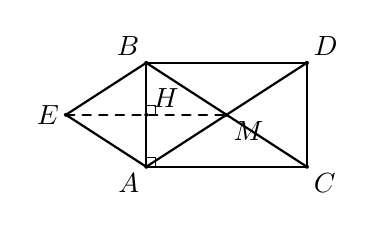
\begin{tikzpicture}[scale=0.60, >=stealth, line join=round, line cap=round]
  \coordinate (A) at (0, 0);
  \coordinate (B) at (0, 2.2);
  \coordinate (C) at (3.4, 0);
  \coordinate (D) at (3.4, 2.2);
  \coordinate (M) at (1.7, 1.1);
  \coordinate (H) at (0, 1.1);
  \coordinate (E) at (-1.7, 1.1);
  \draw[thick] (A) -- (B) -- (D) -- (C) -- cycle;
  \draw[thick] (B) -- (C);
  \draw[thick] (A) -- (D);
  \draw[thick] (B) -- (E) -- (A);
  \draw[thick, dashed] (E) -- (M);
  \draw (0, 0.2) -- (0.2, 0.2) -- (0.2, 0);
  \draw (0, 1.3) -- (0.2, 1.3) -- (0.2, 1.1);
  \fill (A) circle (1.2pt) node[below left=-1pt] {$A$};
  \fill (B) circle (1.2pt) node[above left=-1pt] {$B$};
  \fill (C) circle (1.2pt) node[below right=-1pt] {$C$};
  \fill (D) circle (1.2pt) node[above right=-1pt] {$D$};
  \fill (M) circle (1.2pt) node[below right=-1pt] {$M$};
  \fill (H) circle (1.2pt) node[above right=-1pt] {$H$};
  \fill (E) circle (1.2pt) node[left=-1pt] {$E$};
\end{tikzpicture}
\end{minipage}\par
\vspace{0.4mm}
\noindent\textit{Bài giải:}\dongkeHaiCot{11}
\\ \hline
\end{tabularx}

\vspace{1.4mm}

\noindent
\begin{tabularx}{\linewidth}{|X|}
\hline
\vspace{0.5mm}
\textbf{Câu 14 (0,5 điểm).} Tìm giá trị nhỏ nhất của biểu thức: $A = x^2 - 6x + 2033$.\par
\vspace{0.4mm}
\noindent\textit{Bài giải:}\dongkeHaiCot{7}
\\ \hline
\end{tabularx}

\newpage
% =============================================================================
% ========================= TOAN 8 TUAN 09 BUOI 01 - MA DE 102 =================
% ========================= TRANG 1/2 ==========================================
% =============================================================================
\noindent
\begin{tabularx}{\linewidth}{|X|c|}
\hline
\textbf{PHIẾU KIỂM TRA ĐỊNH KỲ TOÁN 8 - TUẦN 09 - BUỔI 01} & \textbf{Mã đề: 102 - Trang 1/2} \\
\hline
\end{tabularx}

\vspace{1.2mm}

\noindent
\begin{tabularx}{\linewidth}{|p{3.2cm}|X|}
\hline
\centering\textbf{ĐIỂM SỐ} & \centering\textbf{LỜI NHẬN XÉT CỦA THẦY CÔ} \tabularnewline
\hline
\rule{0pt}{1.8cm} & \tabularnewline
\hline
\end{tabularx}

\vspace{1.4mm}
\noindent\textbf{Câu 1 (0,25 điểm).} Bậc của đơn thức $B = 5x^2 y^4 z^2$ là: \shortans{8}\par\vspace{2.3mm}
\noindent\textbf{Câu 2 (0,25 điểm).} Bậc của đa thức $Q = 4x^2 y^2 - 5x^3 - 4x^2 y^2 + 2x^3 + 9$ là: \shortans{3}\par\vspace{2.3mm}
\noindent\textbf{Câu 3 (0,25 điểm).} Giá trị của $N = 3x^2 y - 2xy$ tại $x=1, y=-3$ bằng: \shortans{-3}\par\vspace{2.3mm}
\noindent\textbf{Câu 4 (0,25 điểm).} Cho khai triển $(x-6)^2 = x^2 - bx + 36$. Giá trị của $b$ là: \shortans{12}\par\vspace{2.3mm}
\noindent\textbf{Câu 5 (0,25 điểm).} Tính nhanh giá trị biểu thức $65^2 - 35^2 = $: \shortans{3\,000}\par\vspace{2.3mm}
\noindent\textbf{Câu 6 (0,25 điểm).} Kết quả phép chia $(15x^4 y^3 - 10x^3 y^2) : (5x^3 y^2)$ là: \shortans{3xy - 2}\par\vspace{2.3mm}
\noindent\textbf{Câu 7 (0,25 điểm).} Tứ giác $ABCD$ có $\widehat{A}=70^\circ, \widehat{B}=120^\circ, \widehat{C}=85^\circ$. Số đo góc $D$ là: \shortans{85^\circ}\par\vspace{2.3mm}
\noindent\textbf{Câu 8 (0,25 điểm).} Hình thang cân $ABCD$ ($AB \parallel CD$) có $\widehat{C}=65^\circ$. Số đo góc $A$ là: \shortans{115^\circ}\par\vspace{2.3mm}
\noindent\textbf{Câu 9 (0,25 điểm).} Hình bình hành có một góc vuông là hình gì?: \shortans{Hình chữ nhật}\par\vspace{2.3mm}
\noindent\textbf{Câu 10 (0,25 điểm).} Tam giác vuông có cạnh huyền dài $20\text{ cm}$. Trung tuyến ứng cạnh huyền dài: \shortans{10\text{ cm}}\par\vspace{2.3mm}
\vspace{0.2mm}
\noindent\textbf{Câu 11 (3,0 điểm). Thực hiện phép tính (rút gọn nếu có thể):}
\vspace{0.8mm}

\noindent
\begin{tabularx}{\linewidth}{|X|X|}
\hline
\oBaiTap[5]{a) (0,5 điểm)}{$3x(2x^2 - 3x + 2)$} & 
\oBaiTap[5]{b) (0,5 điểm)}{$(x - 3)(x + 4) - x^2$} \\
\hline
\oBaiTap[5]{c) (0,5 điểm)}{$(x + 4)^2 - (x - 4)^2$} & 
\oBaiTap[5]{d) (0,5 điểm)}{$(18x^4 y^2 - 12x^3 y^3 + 6x^3 y^2) : (6x^3 y^2)$} \\
\hline
\oBaiTap[5]{e) (0,5 điểm)}{$(3x + 1)^2 - 6x(x + 1) - 3x^2$} & 
\oBaiTap[5]{f) (0,5 điểm)}{Cho $B = x^3 + 3x^2 + 3x + 1$. Tính giá trị của $B$ tại $x = 99$.} \\
\hline
\end{tabularx}

\newpage
% =============================================================================
% ========================= TOAN 8 TUAN 09 BUOI 01 - MA DE 102 =================
% ========================= TRANG 2/2 ==========================================
% =============================================================================
\noindent
\begin{tabularx}{\linewidth}{|X|c|}
\hline
\textbf{TOÁN 8 - TUẦN 09 - BUỔI 01} & \textbf{Mã đề: 102 - Trang 2/2} \\
\hline
\end{tabularx}

\vspace{1.4mm}

\noindent\textbf{Câu 12 (2,0 điểm). Tìm số thực $x$, biết:}
\vspace{0.8mm}

\noindent
\begin{tabularx}{\linewidth}{|X|X|}
\hline
\oBaiTap[5]{a) (0,5 điểm)}{$4x(x - 3) - 4x^2 = -24$} & 
\oBaiTap[5]{b) (0,5 điểm)}{$x(x - 5) + 2(x - 5) = 0$} \\
\hline
\oBaiTap[5]{c) (0,5 điểm)}{$(x + 3)^2 - 25 = 0$} & 
\oBaiTap[5]{d) (0,5 điểm)}{$(2x + 1)^2 = 49$} \\
\hline
\end{tabularx}

\vspace{1.4mm}

\noindent
\begin{tabularx}{\linewidth}{|X|}
\hline
\vspace{0.5mm}
\begin{minipage}[t]{0.64\linewidth}
\vspace{0pt}
\textbf{Câu 13 (2,0 điểm).} Cho tam giác $ABC$ vuông tại $A$ ($AB < AC$), đường trung tuyến $AM$. Gọi $D$ là điểm đối xứng với $A$ qua $M$. Gọi $K$ là trung điểm của $AC$, lấy điểm $F$ đối xứng với $M$ qua $K$.\par\vspace{0.4mm}
\textbf{a)} (1,0 điểm) Chứng minh tứ giác $ABDC$ là hình chữ nhật.\par\vspace{0.4mm}
\textbf{b)} (1,0 điểm) Chứng minh tứ giác $AMCF$ là hình thoi.
\end{minipage}\hfill
\begin{minipage}[t]{0.34\linewidth}
\vspace{0pt}\centering
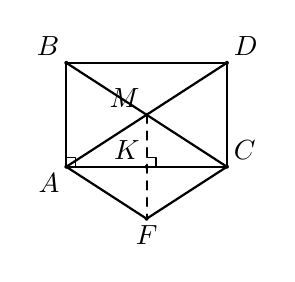
\begin{tikzpicture}[scale=0.60, >=stealth, line join=round, line cap=round]
  \coordinate (A) at (0, 0);
  \coordinate (B) at (0, 2.2);
  \coordinate (C) at (3.4, 0);
  \coordinate (D) at (3.4, 2.2);
  \coordinate (M) at (1.7, 1.1);
  \coordinate (K) at (1.7, 0);
  \coordinate (F) at (1.7, -1.1);
  \draw[thick] (A) -- (B) -- (D) -- (C) -- cycle;
  \draw[thick] (B) -- (C);
  \draw[thick] (A) -- (D);
  \draw[thick] (A) -- (F) -- (C);
  \draw[thick, dashed] (M) -- (F);
  \draw (0, 0.2) -- (0.2, 0.2) -- (0.2, 0);
  \draw (1.7, 0.2) -- (1.9, 0.2) -- (1.9, 0);
  \fill (A) circle (1.2pt) node[below left=-1pt] {$A$};
  \fill (B) circle (1.2pt) node[above left=-1pt] {$B$};
  \fill (C) circle (1.2pt) node[above right=-1pt] {$C$};
  \fill (D) circle (1.2pt) node[above right=-1pt] {$D$};
  \fill (M) circle (1.2pt) node[above left=-1pt] {$M$};
  \fill (K) circle (1.2pt) node[above left=-1pt] {$K$};
  \fill (F) circle (1.2pt) node[below=-1pt] {$F$};
\end{tikzpicture}
\end{minipage}\par
\vspace{0.4mm}
\noindent\textit{Bài giải:}\dongkeHaiCot{11}
\\ \hline
\end{tabularx}

\vspace{1.4mm}

\noindent
\begin{tabularx}{\linewidth}{|X|}
\hline
\vspace{0.5mm}
\textbf{Câu 14 (0,5 điểm).} Tìm giá trị nhỏ nhất của biểu thức: $B = x^2 - 8x + 2041$.\par
\vspace{0.4mm}
\noindent\textit{Bài giải:}\dongkeHaiCot{7}
\\ \hline
\end{tabularx}

\newpage
% =============================================================================
% ========================= TOAN 8 TUAN 09 BUOI 01 - MA DE 103 =================
% ========================= TRANG 1/2 ==========================================
% =============================================================================
\noindent
\begin{tabularx}{\linewidth}{|X|c|}
\hline
\textbf{PHIẾU KIỂM TRA ĐỊNH KỲ TOÁN 8 - TUẦN 09 - BUỔI 01} & \textbf{Mã đề: 103 - Trang 1/2} \\
\hline
\end{tabularx}

\vspace{1.2mm}

\noindent
\begin{tabularx}{\linewidth}{|p{3.2cm}|X|}
\hline
\centering\textbf{ĐIỂM SỐ} & \centering\textbf{LỜI NHẬN XÉT CỦA THẦY CÔ} \tabularnewline
\hline
\rule{0pt}{1.8cm} & \tabularnewline
\hline
\end{tabularx}

\vspace{1.4mm}
\noindent\textbf{Câu 1 (0,25 điểm).} Bậc của đơn thức $C = -6x^4 y z^4$ là: \shortans{9}\par\vspace{2.3mm}
\noindent\textbf{Câu 2 (0,25 điểm).} Bậc của đa thức $R = 5x^4 y - 3x^2 y^2 - 5x^4 y + x^2 y^2 - 1$ là: \shortans{4}\par\vspace{2.3mm}
\noindent\textbf{Câu 3 (0,25 điểm).} Giá trị của $P = 2xy^2 - 3xy$ tại $x=-1, y=2$ bằng: \shortans{-2}\par\vspace{2.3mm}
\noindent\textbf{Câu 4 (0,25 điểm).} Cho khai triển $(2x+1)^2 = 4x^2 + cx + 1$. Giá trị của $c$ là: \shortans{4}\par\vspace{2.3mm}
\noindent\textbf{Câu 5 (0,25 điểm).} Tính nhanh giá trị biểu thức $85^2 - 15^2 = $: \shortans{7\,000}\par\vspace{2.3mm}
\noindent\textbf{Câu 6 (0,25 điểm).} Kết quả phép chia $(18x^3 y^3 - 12x^2 y^2) : (6x^2 y^2)$ là: \shortans{3xy - 2}\par\vspace{2.3mm}
\noindent\textbf{Câu 7 (0,25 điểm).} Tứ giác $ABCD$ có $\widehat{A}=65^\circ, \widehat{B}=115^\circ, \widehat{C}=90^\circ$. Số đo góc $D$ là: \shortans{90^\circ}\par\vspace{2.3mm}
\noindent\textbf{Câu 8 (0,25 điểm).} Hình thang cân $ABCD$ ($AB \parallel CD$) có $\widehat{C}=75^\circ$. Số đo góc $A$ là: \shortans{105^\circ}\par\vspace{2.3mm}
\noindent\textbf{Câu 9 (0,25 điểm).} Hình bình hành có 2 đường chéo bằng nhau là hình gì?: \shortans{Hình chữ nhật}\par\vspace{2.3mm}
\noindent\textbf{Câu 10 (0,25 điểm).} Tam giác vuông có cạnh huyền dài $18\text{ cm}$. Trung tuyến ứng cạnh huyền dài: \shortans{9\text{ cm}}\par\vspace{2.3mm}
\vspace{0.2mm}
\noindent\textbf{Câu 11 (3,0 điểm). Thực hiện phép tính (rút gọn nếu có thể):}
\vspace{0.8mm}

\noindent
\begin{tabularx}{\linewidth}{|X|X|}
\hline
\oBaiTap[5]{a) (0,5 điểm)}{$4x(2x^2 - x + 3)$} & 
\oBaiTap[5]{b) (0,5 điểm)}{$(x - 4)(x + 5) - x^2$} \\
\hline
\oBaiTap[5]{c) (0,5 điểm)}{$(x + 5)^2 - (x - 5)^2$} & 
\oBaiTap[5]{d) (0,5 điểm)}{$(20x^3 y^3 - 15x^2 y^4 + 10x^2 y^3) : (5x^2 y^3)$} \\
\hline
\oBaiTap[5]{e) (0,5 điểm)}{$(2x - 1)^2 - 4x(x - 1)$} & 
\oBaiTap[5]{f) (0,5 điểm)}{Cho $C = x^3 - 6x^2 + 12x - 8$. Tính giá trị của $C$ tại $x = 102$.} \\
\hline
\end{tabularx}

\newpage
% =============================================================================
% ========================= TOAN 8 TUAN 09 BUOI 01 - MA DE 103 =================
% ========================= TRANG 2/2 ==========================================
% =============================================================================
\noindent
\begin{tabularx}{\linewidth}{|X|c|}
\hline
\textbf{TOÁN 8 - TUẦN 09 - BUỔI 01} & \textbf{Mã đề: 103 - Trang 2/2} \\
\hline
\end{tabularx}

\vspace{1.4mm}

\noindent\textbf{Câu 12 (2,0 điểm). Tìm số thực $x$, biết:}
\vspace{0.8mm}

\noindent
\begin{tabularx}{\linewidth}{|X|X|}
\hline
\oBaiTap[5]{a) (0,5 điểm)}{$2x(x - 4) - 2x^2 = -16$} & 
\oBaiTap[5]{b) (0,5 điểm)}{$x(x - 6) + 4(x - 6) = 0$} \\
\hline
\oBaiTap[5]{c) (0,5 điểm)}{$(x + 1)^2 - 36 = 0$} & 
\oBaiTap[5]{d) (0,5 điểm)}{$(3x - 1)^2 = 64$} \\
\hline
\end{tabularx}

\vspace{1.4mm}

\noindent
\begin{tabularx}{\linewidth}{|X|}
\hline
\vspace{0.5mm}
\begin{minipage}[t]{0.64\linewidth}
\vspace{0pt}
\textbf{Câu 13 (2,0 điểm).} Cho tam giác $ABC$ vuông tại $A$ ($AB < AC$), đường trung tuyến $AM$. Gọi $D$ là điểm đối xứng với $A$ qua $M$. Gọi $H$ là trung điểm của $AB$, lấy điểm $E$ đối xứng với $M$ qua $H$.\par\vspace{0.4mm}
\textbf{a)} (1,0 điểm) Chứng minh tứ giác $ABDC$ là hình chữ nhật.\par\vspace{0.4mm}
\textbf{b)} (1,0 điểm) Chứng minh tứ giác $AMBE$ là hình thoi.
\end{minipage}\hfill
\begin{minipage}[t]{0.34\linewidth}
\vspace{0pt}\centering
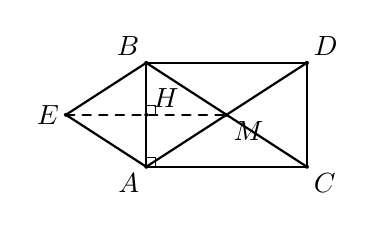
\begin{tikzpicture}[scale=0.60, >=stealth, line join=round, line cap=round]
  \coordinate (A) at (0, 0);
  \coordinate (B) at (0, 2.2);
  \coordinate (C) at (3.4, 0);
  \coordinate (D) at (3.4, 2.2);
  \coordinate (M) at (1.7, 1.1);
  \coordinate (H) at (0, 1.1);
  \coordinate (E) at (-1.7, 1.1);
  \draw[thick] (A) -- (B) -- (D) -- (C) -- cycle;
  \draw[thick] (B) -- (C);
  \draw[thick] (A) -- (D);
  \draw[thick] (B) -- (E) -- (A);
  \draw[thick, dashed] (E) -- (M);
  \draw (0, 0.2) -- (0.2, 0.2) -- (0.2, 0);
  \draw (0, 1.3) -- (0.2, 1.3) -- (0.2, 1.1);
  \fill (A) circle (1.2pt) node[below left=-1pt] {$A$};
  \fill (B) circle (1.2pt) node[above left=-1pt] {$B$};
  \fill (C) circle (1.2pt) node[below right=-1pt] {$C$};
  \fill (D) circle (1.2pt) node[above right=-1pt] {$D$};
  \fill (M) circle (1.2pt) node[below right=-1pt] {$M$};
  \fill (H) circle (1.2pt) node[above right=-1pt] {$H$};
  \fill (E) circle (1.2pt) node[left=-1pt] {$E$};
\end{tikzpicture}
\end{minipage}\par
\vspace{0.4mm}
\noindent\textit{Bài giải:}\dongkeHaiCot{11}
\\ \hline
\end{tabularx}

\vspace{1.4mm}

\noindent
\begin{tabularx}{\linewidth}{|X|}
\hline
\vspace{0.5mm}
\textbf{Câu 14 (0,5 điểm).} Tìm giá trị nhỏ nhất của biểu thức: $C = x^2 - 4x + 2030$.\par
\vspace{0.4mm}
\noindent\textit{Bài giải:}\dongkeHaiCot{7}
\\ \hline
\end{tabularx}

\newpage
% =============================================================================
% ========================= TOAN 8 TUAN 09 BUOI 01 - MA DE 104 =================
% ========================= TRANG 1/2 ==========================================
% =============================================================================
\noindent
\begin{tabularx}{\linewidth}{|X|c|}
\hline
\textbf{PHIẾU KIỂM TRA ĐỊNH KỲ TOÁN 8 - TUẦN 09 - BUỔI 01} & \textbf{Mã đề: 104 - Trang 1/2} \\
\hline
\end{tabularx}

\vspace{1.2mm}

\noindent
\begin{tabularx}{\linewidth}{|p{3.2cm}|X|}
\hline
\centering\textbf{ĐIỂM SỐ} & \centering\textbf{LỜI NHẬN XÉT CỦA THẦY CÔ} \tabularnewline
\hline
\rule{0pt}{1.8cm} & \tabularnewline
\hline
\end{tabularx}

\vspace{1.4mm}
\noindent\textbf{Câu 1 (0,25 điểm).} Bậc của đơn thức $D = 3x^3 y^3 z^2$ là: \shortans{8}\par\vspace{2.3mm}
\noindent\textbf{Câu 2 (0,25 điểm).} Bậc của đa thức $S = 2x^3 y^2 - 4xy^3 - 2x^3 y^2 + 7xy^3 + 6$ là: \shortans{4}\par\vspace{2.3mm}
\noindent\textbf{Câu 3 (0,25 điểm).} Giá trị của $Q = x^2 y - 4xy$ tại $x=-2, y=1$ bằng: \shortans{12}\par\vspace{2.3mm}
\noindent\textbf{Câu 4 (0,25 điểm).} Cho khai triển $(3x-1)^2 = 9x^2 - dx + 1$. Giá trị của $d$ là: \shortans{6}\par\vspace{2.3mm}
\noindent\textbf{Câu 5 (0,25 điểm).} Tính nhanh giá trị biểu thức $55^2 - 45^2 = $: \shortans{1\,000}\par\vspace{2.3mm}
\noindent\textbf{Câu 6 (0,25 điểm).} Kết quả phép chia $(14x^4 y^2 - 7x^3 y) : (7x^3 y)$ là: \shortans{2xy - 1}\par\vspace{2.3mm}
\noindent\textbf{Câu 7 (0,25 điểm).} Tứ giác $ABCD$ có $\widehat{A}=85^\circ, \widehat{B}=105^\circ, \widehat{C}=70^\circ$. Số đo góc $D$ là: \shortans{100^\circ}\par\vspace{2.3mm}
\noindent\textbf{Câu 8 (0,25 điểm).} Hình thang cân $ABCD$ ($AB \parallel CD$) có $\widehat{C}=80^\circ$. Số đo góc $A$ là: \shortans{100^\circ}\par\vspace{2.3mm}
\noindent\textbf{Câu 9 (0,25 điểm).} Tứ giác có các cạnh đối song song là hình gì?: \shortans{Hình bình hành}\par\vspace{2.3mm}
\noindent\textbf{Câu 10 (0,25 điểm).} Tam giác vuông có cạnh huyền dài $24\text{ cm}$. Trung tuyến ứng cạnh huyền dài: \shortans{12\text{ cm}}\par\vspace{2.3mm}
\vspace{0.2mm}
\noindent\textbf{Câu 11 (3,0 điểm). Thực hiện phép tính (rút gọn nếu có thể):}
\vspace{0.8mm}

\noindent
\begin{tabularx}{\linewidth}{|X|X|}
\hline
\oBaiTap[5]{a) (0,5 điểm)}{$5x(2x^2 - 3x + 1)$} & 
\oBaiTap[5]{b) (0,5 điểm)}{$(x - 5)(x + 6) - x^2$} \\
\hline
\oBaiTap[5]{c) (0,5 điểm)}{$(x + 2)^2 - (x - 2)^2$} & 
\oBaiTap[5]{d) (0,5 điểm)}{$(24x^4 y^3 - 16x^3 y^4 + 8x^3 y^3) : (8x^3 y^3)$} \\
\hline
\oBaiTap[5]{e) (0,5 điểm)}{$(3x - 1)^2 - 9x(x - 1) - 3x$} & 
\oBaiTap[5]{f) (0,5 điểm)}{Cho $D = x^3 + 6x^2 + 12x + 8$. Tính giá trị của $D$ tại $x = 98$.} \\
\hline
\end{tabularx}

\newpage
% =============================================================================
% ========================= TOAN 8 TUAN 09 BUOI 01 - MA DE 104 =================
% ========================= TRANG 2/2 ==========================================
% =============================================================================
\noindent
\begin{tabularx}{\linewidth}{|X|c|}
\hline
\textbf{TOÁN 8 - TUẦN 09 - BUỔI 01} & \textbf{Mã đề: 104 - Trang 2/2} \\
\hline
\end{tabularx}

\vspace{1.4mm}

\noindent\textbf{Câu 12 (2,0 điểm). Tìm số thực $x$, biết:}
\vspace{0.8mm}

\noindent
\begin{tabularx}{\linewidth}{|X|X|}
\hline
\oBaiTap[5]{a) (0,5 điểm)}{$5x(x - 2) - 5x^2 = -30$} & 
\oBaiTap[5]{b) (0,5 điểm)}{$x(x - 7) + 3(x - 7) = 0$} \\
\hline
\oBaiTap[5]{c) (0,5 điểm)}{$(x + 4)^2 - 49 = 0$} & 
\oBaiTap[5]{d) (0,5 điểm)}{$(3x + 2)^2 = 25$} \\
\hline
\end{tabularx}

\vspace{1.4mm}

\noindent
\begin{tabularx}{\linewidth}{|X|}
\hline
\vspace{0.5mm}
\begin{minipage}[t]{0.64\linewidth}
\vspace{0pt}
\textbf{Câu 13 (2,0 điểm).} Cho tam giác $ABC$ vuông tại $A$ ($AB < AC$), đường trung tuyến $AM$. Gọi $D$ là điểm đối xứng với $A$ qua $M$. Gọi $K$ là trung điểm của $AC$, lấy điểm $F$ đối xứng với $M$ qua $K$.\par\vspace{0.4mm}
\textbf{a)} (1,0 điểm) Chứng minh tứ giác $ABDC$ là hình chữ nhật.\par\vspace{0.4mm}
\textbf{b)} (1,0 điểm) Chứng minh tứ giác $AMCF$ là hình thoi.
\end{minipage}\hfill
\begin{minipage}[t]{0.34\linewidth}
\vspace{0pt}\centering
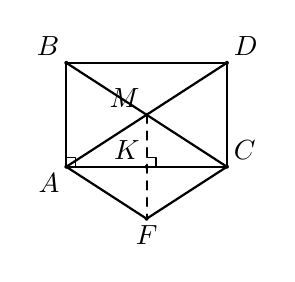
\begin{tikzpicture}[scale=0.60, >=stealth, line join=round, line cap=round]
  \coordinate (A) at (0, 0);
  \coordinate (B) at (0, 2.2);
  \coordinate (C) at (3.4, 0);
  \coordinate (D) at (3.4, 2.2);
  \coordinate (M) at (1.7, 1.1);
  \coordinate (K) at (1.7, 0);
  \coordinate (F) at (1.7, -1.1);
  \draw[thick] (A) -- (B) -- (D) -- (C) -- cycle;
  \draw[thick] (B) -- (C);
  \draw[thick] (A) -- (D);
  \draw[thick] (A) -- (F) -- (C);
  \draw[thick, dashed] (M) -- (F);
  \draw (0, 0.2) -- (0.2, 0.2) -- (0.2, 0);
  \draw (1.7, 0.2) -- (1.9, 0.2) -- (1.9, 0);
  \fill (A) circle (1.2pt) node[below left=-1pt] {$A$};
  \fill (B) circle (1.2pt) node[above left=-1pt] {$B$};
  \fill (C) circle (1.2pt) node[above right=-1pt] {$C$};
  \fill (D) circle (1.2pt) node[above right=-1pt] {$D$};
  \fill (M) circle (1.2pt) node[above left=-1pt] {$M$};
  \fill (K) circle (1.2pt) node[above left=-1pt] {$K$};
  \fill (F) circle (1.2pt) node[below=-1pt] {$F$};
\end{tikzpicture}
\end{minipage}\par
\vspace{0.4mm}
\noindent\textit{Bài giải:}\dongkeHaiCot{11}
\\ \hline
\end{tabularx}

\vspace{1.4mm}

\noindent
\begin{tabularx}{\linewidth}{|X|}
\hline
\vspace{0.5mm}
\textbf{Câu 14 (0,5 điểm).} Tìm giá trị nhỏ nhất của biểu thức: $D = x^2 - 10x + 2052$.\par
\vspace{0.4mm}
\noindent\textit{Bài giải:}\dongkeHaiCot{7}
\\ \hline
\end{tabularx}
\end{document}
